\section{More Expressive Models of Recommmendation Graphs}

Having described the fixed-degree model in detail above, we can now
use it as a template for the analysis of three more richer, more
expressive and realistic models. In practice, websites can not pick
edges uniformly at random from all the other pages on the site. There
are natural clusters of pages so that pages within the clusters are
more closely related than those outside. 

This is the motivation to extend our previous analysis to the cases
when the underlying graph has substructure.  In
Section~\ref{hierarchy}, we analyze the {\em hierarchical tree model}
which models graphs that contain natural tree like clusters.  In
Section~\ref{weighted}, we generalize to the {\em cartesian product model}
where edge density may vary across different pairs of
categories. Finally, in Section~\ref{weighted} we study the {\em
  weighted model} which assigns weights to the graph so that we can
incorporate traffic patterns across a website.

\subsection{Hierarchical Tree Model}
\label{hierarchy}
In this section we explore the hierarchical tree model. We will assume
that we are given a bipartite graph $G=(L,R,E)$. The vertex sets $L$
and $R$ are the leaf sets of two full binary trees $T_L$ and $T_R$ of
depth $D$ where there is a one-to-one correspondence between the
subtrees of these two trees. We also assume that each branching in
both $T_L$ and $T_R$ splits the nodes evenly into the two
subtrees. As in the previous sections, we set $|L|/|R|=k$, but we also
note that this ratio still holds if we take any subtree on the left 
and its corresponding subtree on the right. By abuse of notation, we 
will use a subtree and its leaf set interchangeably. The trees are
fixed in advance, but $G$ is generated probabilistically according to
the following procedure. Let $u\in L$ and $T_L^0, \ldots T^{D-1}_L$ be
the subtrees it belongs at depths $0,\ldots, D-1$. Also, let 
$T_R^0,\ldots, T_R^{D-1}$ be the subtrees on the right that correspond
to these trees on the left. We let $u$ make an edge to $d_{D-1}$ of
the vertices in $T_{R}^{D-1}$, $d_{D-2}$ edges to the vertices in 
$T_{R}^{D-1} \backslash T_{R}^{D-2}$ and so on. Each vertex is chosen
with uniform probability and we let $d = d_{0} + \ldots + d_{D-1}$.\vs

\begin{figure}[h]
\centering
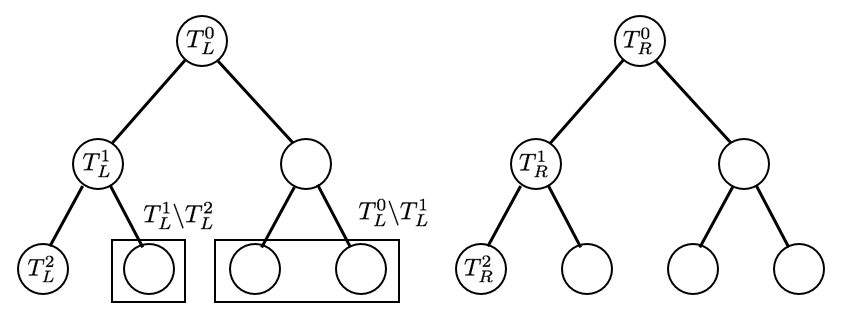
\includegraphics[width=0.6\textwidth]{hierarchy_tree.png}
\begin{minipage}[h]{0.7\textwidth}
\caption{This diagram shows the notation we use for this model and the 1-to-1 correspondance of subtrees}
\end{minipage}
\end{figure}

Our goal now is to find a $b$-matching in this graph that is close to
optimal in expectation. That is, our degree upper bound on vertices in
$L$ is $c$ and the degree lower bound on vertices in $L$ is 1. Let $c
= c_0 + \ldots + c_{D-1}$ similarly to how we defined $d$. 
To combine the analysis of the randomness of the algorithm
and the randomness of the graph, the algorithm will pick $c_{i}$ edges
uniformly from among the $d_{i}$ edges going to each level of the
subtree. This enables us to think of the subgraph our algorithm
outputs as being generated by the graph generation process, but with
fewer neighbors selected for each as in the previous sections. With
this model and parameters in place, we can prove the following
theorem.\

\begin{thm}
Let $S$ be the subset of edges $v\in R$ such that $\deg_H(v) \geq 1$. Then
\[ \E[S] \geq r(1-\exp(-ck)) \]
where the expectation is taken over $G$ and $H$.
\end{thm}

\begin{proof}
Let $v\in R$ and let $T_L^{D-1}, T_L^{D-2}\backslash T_L^{D-1},
\ldots, T_L^0\backslash T_L^1$ be the sets it can take edges
from. Since $T_L$ and $T_R$ split perfectly evenly at each node the
vertices in these sets will be choosing from $r_{D-1}, r_{D-1},
r_{D-2},\ldots, r_{1}$ vertices in $R$ for neighbors respectively,
where $r_i$ is the size of subtree of the right tree rooted at depth
$i$. Furthermore, each of these sets described above have size
$l_{D-1}, l_{D-1}, l_{D-2}, \ldots, l_{1}$ respectively, where $l_i$
is the size of a subtree of $T_L$ rooted at depth $i$. It follows that
the probability that $v$ does not receive any edges at all is at most

\begin{align*}
	      \Pr[\lnot X_v] 
	&=    \left(1-\frac{1}{r_{D-1}}\right)^{c_0l_{D-1}}\prod_{i=1}^{D-1}\left(1 - \frac{1}{r_i}\right)^{c_{D-i} l_i} \\
	&\leq \exp\left(-\frac{l_{D-1}}{r_{D-1}}c_0\right)\prod_{i=1}^{D-1} \exp\left(-\frac{l_i}{r_i}c_{D-i}\right) \\
	&=    \exp\left(-(c_0 + \ldots + c_{D-1})k\right) \\
	&=    \exp(-ck)
\end{align*}

Since this is an indicator variable, it follows that 
\[ \E[S] = \E\left[\sum_{v \in R} X_v \right] \geq r \left(1-\exp(-ck)\right) \]
\end{proof}

Note that this is the same result as we obtained for the fixed degree
model in Section \ref{fixed-degree}. In fact, the approximation
guarantees when $ck \ll 1$ or $ck \gg 1$ hold exactly as before.\vs

The sampling of $H$ can be done algorithmically because we separated
out the edge generation process at a given depth from the edge
generation process at deeper subtrees. There is no ambiguity as to why
an edge is in the underlying graph. That is, if we superimpose $T_L$
and $T_R$, then an edge between $u_l\in L$ and $v_r\in R$ must have
come from an edge generated at the lowest common ancestor of $u_l$ and
$v_r$. So the algorithm can actually sample intelligently and in the
same way that the graph was generated in the first place. Also note
that we do not have to assume that the trees $T_L$ and $T_R$ are
binary. We only need the trees to be regular and evenly divided at
each vertex since the proof only relies on the proportions of the
sizes of the subtrees in $T_L$ and $T_R$.


\subsection{Cartesian Product Model}
\label{cartesian}
We can extend the analysis in Section \ref{fixed-degree} in a way
orthogonal to the hierarchical tree model as follows. We assume that
$L$ has been partitioned into $t$ subsets $L_1,\ldots, L_t$ and
that $R$ has been partitioned into $t'$ subsets $R_1,\ldots,
R_{t'}$. For convenience, we let $|L_i| = l_i$ and $|R_i|=r_i$. Given
this suppose that for each $1\leq i\leq t$ and each $1\leq j\leq t'$,
$G[L_i, R_j]$ is an instance of the Fixed Degree Model with
$d=d_{ij}$. We assume that for all $i$, we have $\sum_{j=1}^{t'}
d_{ij} = d$ for some fixed $d$. Also assume that we have fixed in
advance $c_{ij}$ for each $1\leq i\leq t$ and $1\leq j\leq t'$ that
satisfy $\sum_{j=1}^{t'} c_{ij} = c$ for all $i$ for some fixed $c$.
To sample $H$ from $G$, we sample $c_{ij}$ neighbors for each 
$u_i\in L_i$ from $R_i$. Letting $S$ be the set of vertices in 
$v\in R$ that satisfy $\deg_H(v)\geq 1$, we can show the following:

\begin{thm}
With $S$, $G$ and $H$ defined as above, we have
\[ \E[S] \geq r - \sum_{j=1}^{t'} r_j \exp\left(-\sum_{i=1}^t c_{ij} \frac{l_i}{r_j}\right)\]
where the expectation is over $G$ and $H$.
\end{thm}
\begin{proof}
Let $v_j \in R_j$ be an arbitrary vertex and let $X_{v_j}$ be the
indicator variable for the event that $\deg_H(v_i) \geq 1$. The
probability that none of the neighbors of some $u_i\in R_i$ is $v_j$
is exactly $(1-\frac{1}{r_j})^{c_{ij}}$. It follows that the
probability that the degree of $v_j$ in the subgraph $H[L_i,R_j]$ is 0
is at most $(1-\frac{1}{r_j})^{c_{ij}l_i}$. Considering this
probability over all $R_j$ gives us:
\[ \Pr[X_{v_i} = 0] = \prod_{i=1}^{t} \left(1-\frac{1}{r_j}\right)^{c_{ij} l_i} \leq \exp\left(-\sum_{i=1}^t c_{ij} \frac{l_i}{r_j}\right)\]

By linearity of expectation $\E[S] = \sum_{i=1}^{t'} r_i \E[X_{v_i}]$,
so it follows that
\[ \E[S] \geq \sum_{j=1}^{t'} r_j \left(1-\exp\left(-\sum_{i=1}^t c_{ij} \frac{l_i}{r_j}\right)\right) = r - \sum_{j=1}^{t'} r_j \exp\left(-\sum_{i=1}^t c_{ij} \frac{l_i}{r_j}\right)\]
\end{proof}

This model is interesting because it can capture a broader set of
recommendation subgraphs than the fixed degree model. However, it is
difficult to estimate how good a solution will be without knowing
the sizes of the sets in the partitions. However, we can note that we
obtain the approximation guarantee of $(1-\exp(-ck))$ provided that
$l_i/r_j = k$ for all $i$ and $j$ where $k$ is some fixed
constant. Another interesting point about this model and the algorithm
we described for sampling $H$ is that we are free to set the $c_{ij}$
as we see fit. In particular, $c_{ij}$ can be chosen to maximize the
approximation guarantee in expectation we obtained above using
gradient descent or some other first order method prior to running the
recommendation algorithm to increases the quality of the solution.


\subsection{Weighted Model}
\label{weighted}
The fixed degree model of Section \ref{fixed-degree} is a simple and
convenient model, but the assumption that all recommendations hold the
same weight is unrealistic. This motivates fixing the graph to be the
complete bipartite graph $K_{l,r}$, and giving the edges i.i.d weights
with mean $\mu$. We modify the objective function accordingly, so that
we count only the vertices in $R$ which have weight $\geq 1$. If we
assume that $ck\mu \geq 1+\epsilon$ for some $\epsilon > 0$, then 
the naive sampling solution we outlined in Section \ref{fixed-degree}
still performs exceptionally well. If we let $S$ be the size of the 
solution produced by this algorithm we have:

\begin{thm}
Let $G=K_{l,r}$ be a bipartite graph where the edges have i.i.d. weights and come from a distribution with mean $\mu$ that is supported on $[0,b]$. If the algorithm from Section \ref{fixed-degree} is used to sample a subgraph $H$ from $G$, then
\[ \E[S] = \sum_{v\in R} \E[X_v] = r\left(1-\exp\left(-\frac{2l\epsilon^2}{b^2}\right)\right) \]
\end{thm}

\begin{proof}
For each edge $uv\in G$, let $W_{uv}$ be its random weight, $Y_{uv}$ be
the indicator for the event $uv\in H$ and define $X_{uv} = Y_{uv}
W_{uv}$. Since weights and edges are sampled by independent processes,
we have $\E[X_{uv}] = \E[W_{uv}]\E[Y_{uv}]$ for all edges. Since $c$
edges out of $r$ are picked for each vertex, $\E[Y_{uv}] = \frac{c}{r}$
, so $\E[X_{uv}] = \frac{c}{r}\mu$. Therefore, the expected weight
coming into a vertex $v\in R$ would be 

\[ \E[X_v] = \sum_{u\in L} \E[X_{uv}] = \frac{cl\mu}{r} = ck\mu\]

However, $X_{uv}$ for each $u$ are i.i.d random variables. Since by
assumption $ck\mu = 1+\epsilon$, by a Hoeffding bound we can obtain:

\[ \Pr[X_v \leq 1] = \Pr[X_v - \E[X_v] \geq \epsilon] \leq \exp\left(-\frac{2l\epsilon^2}{b^2}\right) \]

By linearity of expectation we can now get the result in the theorem

\[ \E[S] = \sum_{v\in R} \E[X_v] = r\left(1-\exp\left(-\frac{2l\epsilon^2}{b^2}\right)\right) \]
\end{proof}

There are two things to note about this variant. The first is that
since the variables $X_v$ are negatively correlated, our results in
\ref{worst-vs-avg} can be readily extended to the results of this
section. The second is that the condition that $W_{uv}$ are i.i.d
is not necessary to obtain the full effect of the analysis. Indeed,
the only place in the proof where the fact that $W_{uv}$ are i.i.d
is when we argued that $X_{uv}$ is large with high probability by a
Hoeffding bound. For the bound to apply, it's sufficient to assume
that $W_{uv}$ for all $v$ are independent. In particular, it's 
possible that $W_{uv}$ for all $u$ are inter-dependent. This allows
us to assume an weight distribution that depends on the strength of 
the recommender and the relevance of the recommendation separately.
